%!TEX root = ../report.tex
\documentclass[../report.tex]{subfiles}
\begin{document}
    \chapter{Evaluation and Results}
	This chapter presents the results of experiments whose implementation details were provided in the last chapter. Besides, the outcomes are systematically analyzed and evaluated.
	
	
	\section{Background}
	We conducted the first three experiments (A. patient-wise attribution map generation, B. composite face generation and C. syndrome-wise attribution map generation) on each of the 139 frequent syndrome classes in the GestaltMatcherDataBase (GMDB) dataset. However, as mentioned earlier, experimental artifacts related to six of the syndromes (Cornelia de Lange syndrome (CDLS), Williams Beuren syndrome (WBS),  Coffin-Siris syndrome (CSS),  Nicolaides-Baraitser syndrome (NBS), Hyperphosphatasia-intellectual disability syndrome or Hyperphosphatasia mental retardation syndrome (HPMRS) and Smith-Lemli-Opitz-Syndrome (SMOS)) were evaluated by an experienced clinical geneticist. The clinician specialized in the diagnosis of three of the syndromes (CDLS, WBS, HPMRS), and had less familiarity with others. Therefore, analyses and discussions on experimental results mostly revolve around the three syndrome categories. Besides, some important findings from other syndromes are also provided. In this section, some background information regarding facial phenotypic features of the syndromes discussed in this chapter is given. 
	
	\subsubsection{Cornelia De Lange Syndrome}
		\begin{figure}[H]\label{fig_cdls_char}
		\centering
		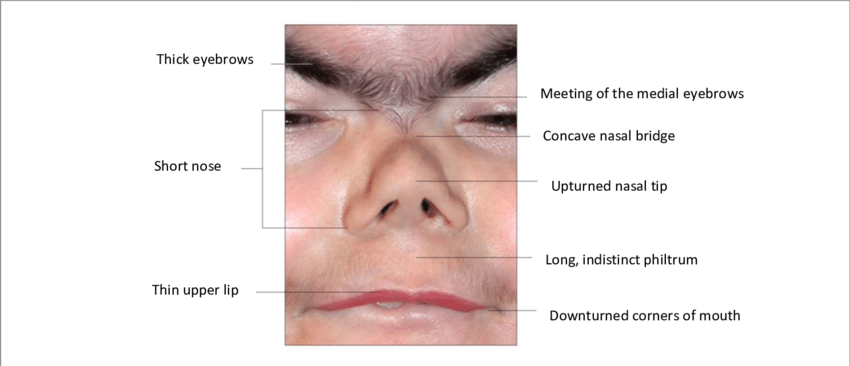
\includegraphics[scale=0.5, trim = 1cm 1cm 1cm 1cm, clip]{chapter6/cdls/cdls_ref.png}	
		\caption[Cardinal features of CDLS]{Cardinal facial features of CDLS. Image source: \cite{kline2018diagnosis}}
	\end{figure}
	
	\begin{figure}[H]\label{fig_cdls}
		\centering
		\begin{subfigure}[t]{0.24\textwidth}
			\centering
			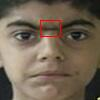
\includegraphics[width=\textwidth]{chapter6/cdls/0_3529.jpg}
			\caption{Synophrys}
		\end{subfigure}
		\begin{subfigure}[t]{0.24\textwidth}
			\centering
			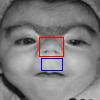
\includegraphics[width=\textwidth]{chapter6/cdls/9_2000.jpg}
			\caption{Depressed nasal bridge (red), long philtrum (blue)}
		\end{subfigure}	
		\begin{subfigure}[t]{0.24\textwidth}
			\centering
			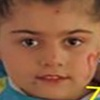
\includegraphics[width=\textwidth]{chapter6/cdls/33_3580.jpg}
			\caption{Thin upper lip}
		\end{subfigure}	
		\begin{subfigure}[t]{0.24\textwidth}
			\centering
			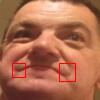
\includegraphics[width=\textwidth]{chapter6/cdls/117_3699.jpg}
			\caption{Down-turned corners of mouth}
		\end{subfigure}
		\caption[Instances of CDLS from GMDB dataset]{Instances of CDLS from GMDB dataset annotated with phenotypic facial features}
	\end{figure}
	
	\subsubsection{Williams Beuren Syndrome}
	
	\begin{figure}[H]\label{fig_williams_char}
	\centering
	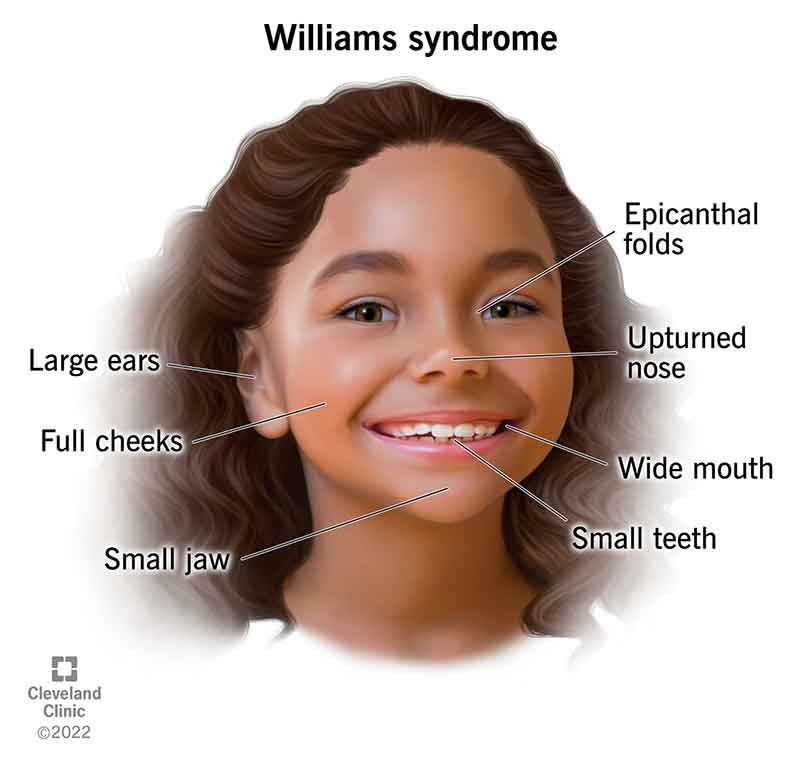
\includegraphics[scale=0.2]{chapter6/william/williams_syndrome_ref.jpg}	
	\caption[An animated characteristic face of WBS]{An animated characteristic face of WBS. Image source: Cleveland clinic \protect\footnotemark.} 
	\end{figure}
	 \footnotetext{Cleveland clinic - \url{https://my.clevelandclinic.org/health/diseases/15174-williams-syndrome}}
	\begin{figure}[H]\label{fig_williams}
		\centering
		\begin{subfigure}[t]{0.24\textwidth}
			\centering
			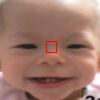
\includegraphics[width=\textwidth]{chapter6/william/4_37.jpg}
			\caption{Depressed nasal bridge}
		\end{subfigure}
		\begin{subfigure}[t]{0.24\textwidth}
			\centering
			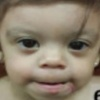
\includegraphics[width=\textwidth]{chapter6/william/4_73.jpg}
			\caption{Long philtrum}
		\end{subfigure}	
			\begin{subfigure}[t]{0.24\textwidth}
			\centering
			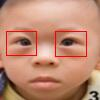
\includegraphics[width=\textwidth]{chapter6/william/130_36.jpg}
			\caption{Puffy eyes}
		\end{subfigure}	
			\begin{subfigure}[t]{0.24\textwidth}
			\centering
			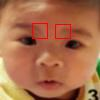
\includegraphics[width=\textwidth]{chapter6/william/164_35.jpg}
			\caption{Medial eyebrow flares}
		\end{subfigure}	
	\caption[Instances of WBS from GMDB dataset]{Instances of WBS from GMDB dataset annotated with phenotypic facial features}
	\end{figure}





	\subsubsection{Hyperphosphatasia with Mental Retardation Syndrome}
	 
	 \begin{figure}[H]\label{fig_hpmrs}
	 	\centering
	 	\begin{subfigure}[t]{0.17\textwidth}
	 		\centering
	 		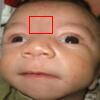
\includegraphics[width=\textwidth]{chapter6/hpmrs/2_499.jpg}
	 		\caption{Hypertelorism}
	 	\end{subfigure}
	 	\begin{subfigure}[t]{0.17\textwidth}
	 		\centering
	 		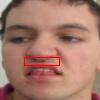
\includegraphics[width=\textwidth]{chapter6/hpmrs/15_1758.jpg}
	 		\caption{Short philtrum}
	 	\end{subfigure}	
	 	\begin{subfigure}[t]{0.17\textwidth}
	 		\centering
	 		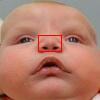
\includegraphics[width=\textwidth]{chapter6/hpmrs/17_1774.jpg}
			\caption{Short nose}
	 	\end{subfigure}	
	 	\begin{subfigure}[t]{0.17\textwidth}
	 		\centering
	 		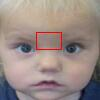
\includegraphics[width=\textwidth]{chapter6/hpmrs/20_888.jpg}
	 		\caption{Broad nasal bridge}
	 	\end{subfigure}	
	 	\begin{subfigure}[t]{0.17\textwidth}
	 		\centering
	 		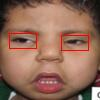
\includegraphics[width=\textwidth]{chapter6/hpmrs/33_1773.jpg}
	 		\caption{Upslanting palpebral fissures}
	 	\end{subfigure}	
	 	\caption[Instances of HPMRS from GMDB dataset]{Instances of HPMRS from GMDB dataset annotated with phenotypic facial features}
	 \end{figure}
	 
	 	\subsubsection{Coffin Siris Syndrome}
	 
	 \begin{figure}[H]\label{fig_cfs}
	 	\centering
	 	\begin{subfigure}[t]{0.17\textwidth}
	 		\centering
	 		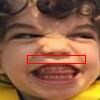
\includegraphics[width=\textwidth]{chapter6/cfs/5_1981.jpg}
	 		\caption{Short philtrum}
	 	\end{subfigure}
	 	\begin{subfigure}[t]{0.17\textwidth}
	 		\centering
	 		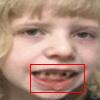
\includegraphics[width=\textwidth]{chapter6/cfs/6_810.jpg}
	 		\caption{Thin upper-lip vermilion and thich lower-lip vermilion }
	 	\end{subfigure}	
	 	\begin{subfigure}[t]{0.17\textwidth}
	 		\centering
	 		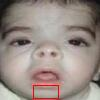
\includegraphics[width=\textwidth]{chapter6/cfs/17_2539.jpg}
	 		\caption{Small chin}
	 	\end{subfigure}	
	 	\begin{subfigure}[t]{0.17\textwidth}
	 		\centering
	 		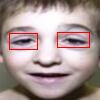
\includegraphics[width=\textwidth]{chapter6/cfs/20_2465.jpg}
	 		\caption{Downslanting palpebral fissures}
	 	\end{subfigure}	
	 	\begin{subfigure}[t]{0.17\textwidth}
	 		\centering
	 		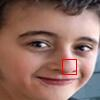
\includegraphics[width=\textwidth]{chapter6/cfs/46_1986.jpg}
	 		\caption{Broad nasal tip}
	 	\end{subfigure}	
	 	\caption[Instances of HPMRS from GMDB dataset]{Instances of CSS from GMDB dataset annotated with phenotypic facial features}
	 \end{figure}
	 
	 
    \section{Experiment A. Patient-wise Attribution Map Generation}
    
    
    
    \subsection{Results from Clinician's Evaluation}
    The clinician was presented with attribution maps of 23 instances from six different syndromes classes in GMDB. However, as mentioned earlier, his specialization was limited to three syndromes which were represented by 15 samples in the questionnaire. Table \ref{tab_cl_acc} shows the sample distribution, and diagnostic performance of the clinician for each syndrome class, without the aid of attribution maps. As described in  Chapter \ref{ch_method}, it is important to note that only samples from the test split of GMDB that were correctly classified by the GestaltMatcher classifier model, were chosen for evaluation. 
    
    
   	\begin{figure}[H]
   	\centering
   	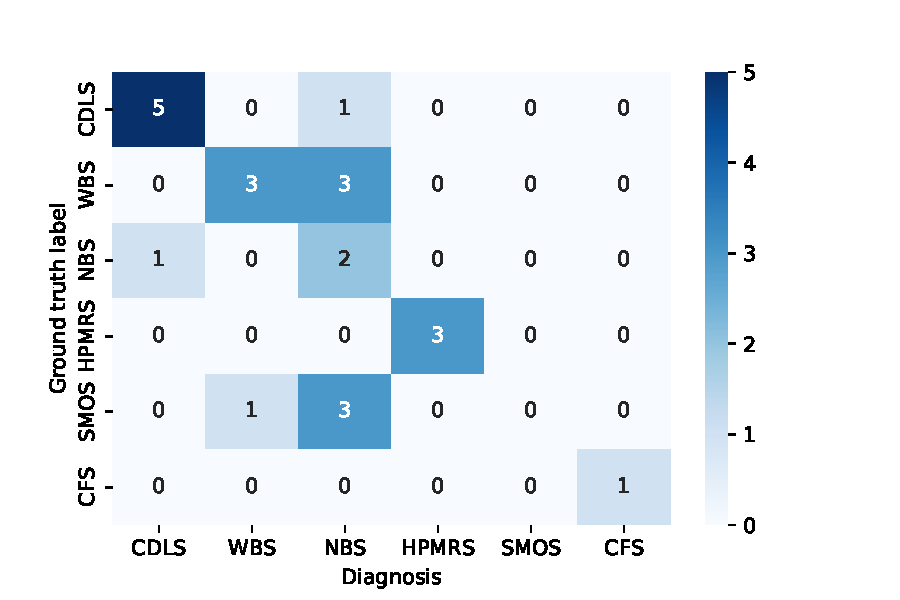
\includegraphics[scale=0.6,trim=0.5cm 0cm 0.5cm 0cm, clip]{chapter6/clinician_conf_matrix.pdf}	
   	\caption[Confusion matrix representing the clinician's
   	diagnostic performance]{Confusion matrix representing the clinician's
   	diagnostic performance}
   \label{fig_clin_perf_mtx} 
   \end{figure}
    

 \begin{table}[H]
 	\begin{tabular}{|c|c|c|c|c|c|c|}
 		\hline
 		\textbf{Syndrome} & \textbf{Sample count} & \textbf{\begin{tabular}[c]{@{}c@{}}Clinician \\ specializes in\\ syndrome\end{tabular}} & \textbf{Precision} & \textbf{Recall} & \multicolumn{1}{l|}{\textbf{F1-score}} & \textbf{Accuracy} \\ \hline
 		\textbf{CDLS}              & 6                     & yes                                                                                     & 0.83               & 0.83            & 0.83                                   & 0.83              \\ \hline
 		\textbf{WBS}               & 6                     & yes                                                                                     & 0.75               & 0.50            & 0.60                                   & 0.50              \\ \hline
 		NBS               & 3                     & no                                                                                      & 0.22               & 0.67            & 0.33                                   & 0.67              \\ \hline
 		\textbf{HPMRS}             & 3                     & yes                                                                                     & 1.00               & 1.00            & 1.00                                   & 1.00              \\ \hline
 		SMOS              & 4                     & no                                                                                      & 0.00               & 0.00            & 0.00                                   & 0.00              \\ \hline
 		CFS               & 1                     & no                                                                                      & 1.00               & 1.00            & 1.00                                   & 1.00              \\ \hline
 	\end{tabular}
 \caption{Diagnostic performance of the clinician on samples in the questionnaire}
  \label{tab_cl_acc}
\end{table}
  \subsubsection{Usefulness of Attribution Maps in Diagnoses}
  Fig \ref{fig_patient_flow} in Chapter \ref{ch_method} enumerated the following possible inferences, which can obtained from responses in the patient-wise attribution map evaluation section of the questionnaire:
  \begin{itemize}
  	\item A. Attribution maps misleads the clinician to make incorrect diagnosis
  	\item B. Attribution maps reinforces the clinician's correct diagnosis
  	\item C. Attribution maps helps the clinician to correct his diagnosis
  	\item D. Attribution maps fail to help the clinician to correct his diagnosis
  \end{itemize} 
  Here, we describe the usefulness of attribution maps and performance of methods used to generate them, by binning clinician responses into one of the above mentioned, and analyzing them. 
  
  As shown in Figure \ref{fig_clin_perf_mtx}, the clinician correctly diagnosed 11 out of the total 15 patient images, presented to him from the syndromes of his specialty, without the aid of attribution maps. His responses to the subsequent questions (Refer questions 2b - 2e in Table \ref{tbl_synd_wise}) asked after the 11 correctly diagnosed cases, indicate that the attribution maps reinforced correct diagnoses (scenario B) in eight cases, and didnot prove helpful (scenario A) in  three. Within the 8 occurrences of scenario B, attribution maps using FullGrad were marked to best highlight the associated facial features in five, followed by the maps of other methods in one each. Among the four misdiagnosed instances, none of the attribution maps proved effective in correcting three of his predictions (scenario D), and a FullGrad attribution map helped him correct one (scenario C). To summarize, the clinician found attribution maps in general, to be helpful for diagnosis in 9 out of 15 instances, and also chose FullGrad maps to highlight relevant facial features in most of the cases.
  \subsubsection{Comparing Attention Regions}
   Besides identifying syndromes and rating attribution maps, the clinician was asked to specify the key facial features which he used for diagnosis (Refer question 2b in \ref{tbl_synd_wise}). From his answers, let us compare his regions of attention with that of the GestaltMatcher classifier model, represented in form of attribution maps.  Figure \ref{fig_match_cl_maps} and Figure \ref{}  contain examples of attribution map sets of correctly diagnosed samples, for which features considered crucial by the clinician, matched and differed with that of the classifer respectively.	
		\begin{figure}[H]
		\centering			
		\begin{subfigure}[t]{1\textwidth}
			\centering
			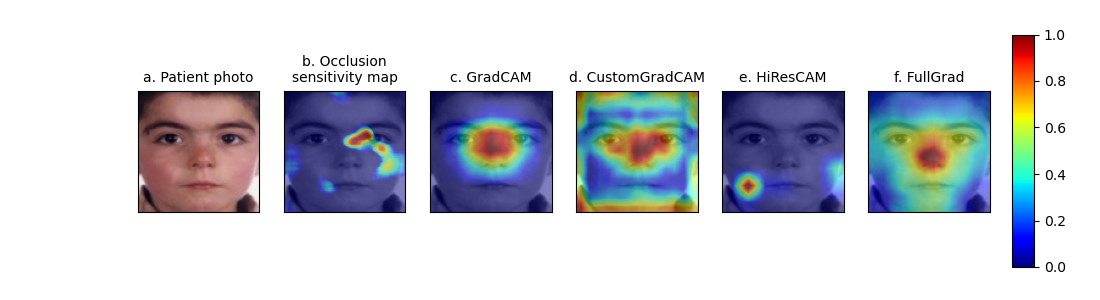
\includegraphics[width=\textwidth, trim = 1cm 2.50cm 1cm 2cm, clip]{chapter6/cdls/0_205.png}
			\caption{Patient with CDLS and eyebrows specified as the key feature}
		\end{subfigure}
		\begin{subfigure}[t]{1\textwidth}
			\centering
			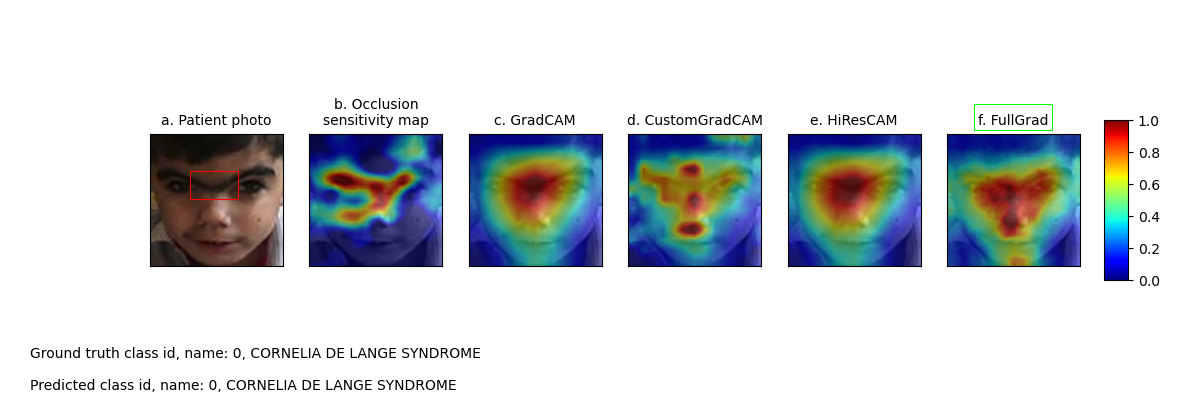
\includegraphics[width=\textwidth, trim = 1cm 2.50cm 1cm 2cm, clip]{chapter6/cdls/4_3556.png}
			\caption{Patient with CDLS and synophrys feature}
		\end{subfigure}
		\begin{subfigure}[t]{1\textwidth}
			\centering
			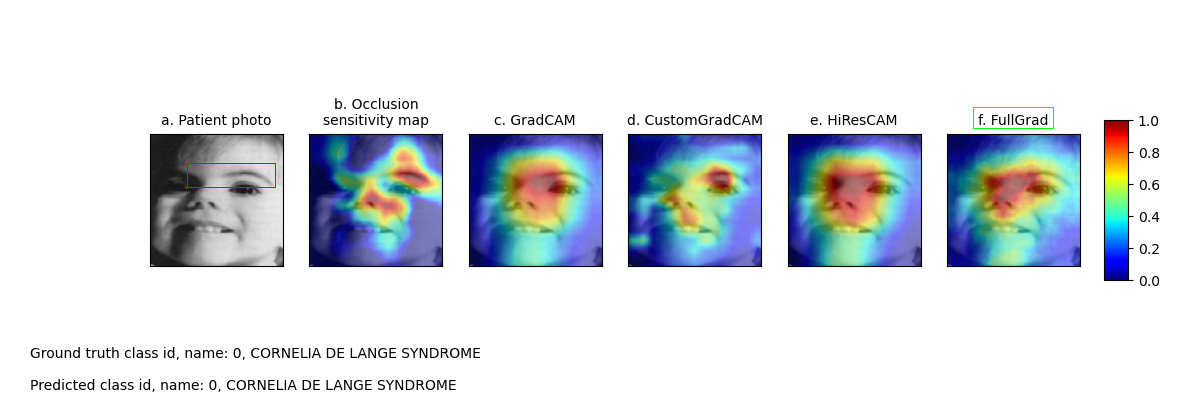
\includegraphics[width=\textwidth, trim = 1cm 2.50cm 1cm 2cm, clip]{chapter6/cdls/6_222.png}
			\caption{Patient with CDLS and eyebrows specified as the key feature}
		\end{subfigure}
		\begin{subfigure}[t]{1\textwidth}
			\centering
			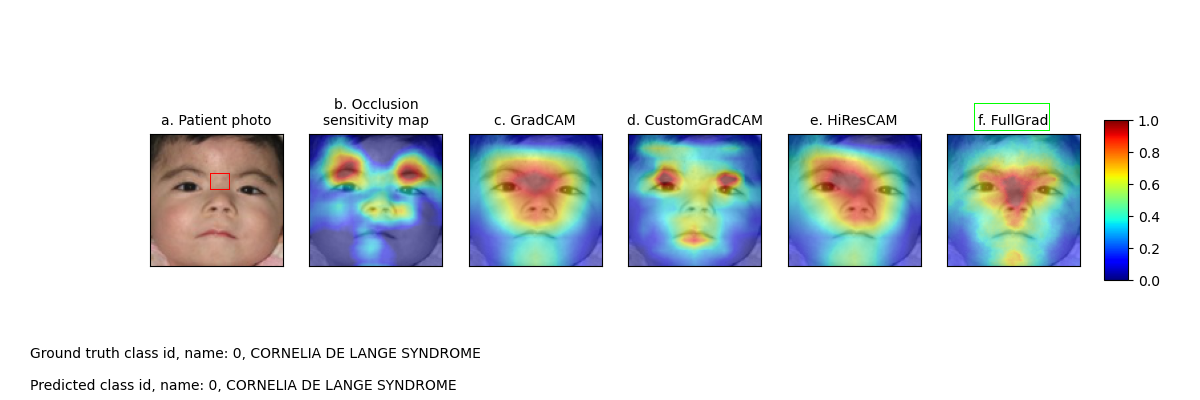
\includegraphics[width=\textwidth, trim = 1cm 2.50cm 1cm 2cm, clip]{chapter6/cdls/7_285.png}
			\caption{Patient with CDLS and nose, depressed nasal bridge reported as the key features}
		\end{subfigure}
		\caption[Attribution maps of instances in which clinician's attention regions differ from that of the classifier model]{Attribution maps of instances in which clinician's attention regions differ from that of the classifier model. Key features specified and methods chosen by the clinician are boxed in red and green colors respectively}
	\label{fig_match_cl_maps}
	\end{figure}
	\begin{figure}[H]
		\begin{subfigure}[t]{1\textwidth}
			\centering
			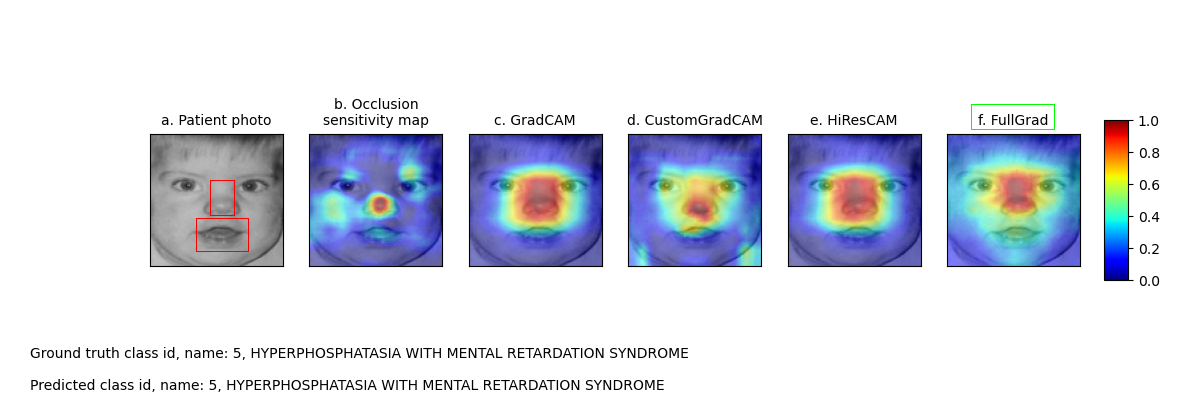
\includegraphics[width=\textwidth, trim = 1cm 2.50cm 1cm 2cm, clip]{chapter6/hpmrs/0_2425.png}
			\caption{Patient with  HPMRS, and nose and mouth specified as key features}
		\end{subfigure}
		\begin{subfigure}[t]{1\textwidth}
			\centering
			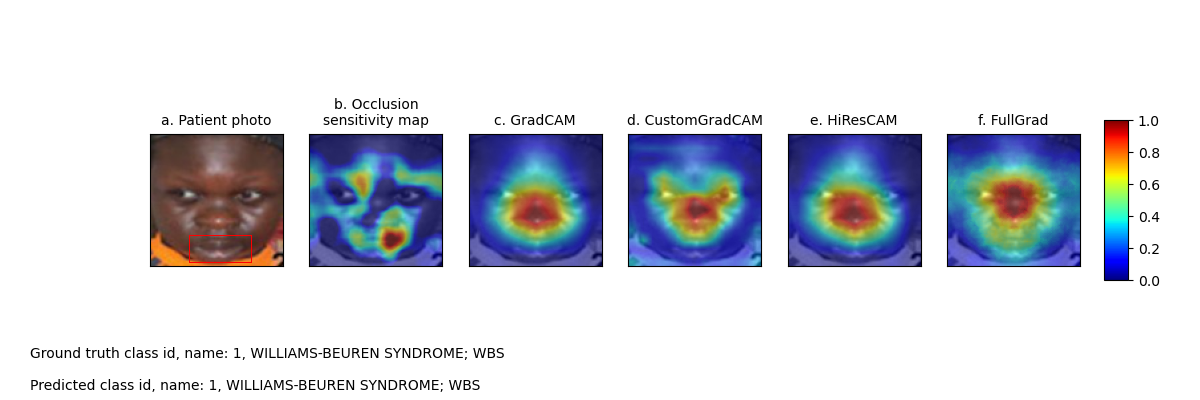
\includegraphics[width=\textwidth, trim = 1cm 2.50cm 1cm 2cm, clip]{chapter6/william/5_31.png}
			\caption{Patient with  WBS, and lips specified as the key feature}
		\end{subfigure}
		\begin{subfigure}[t]{1\textwidth}
		\centering
		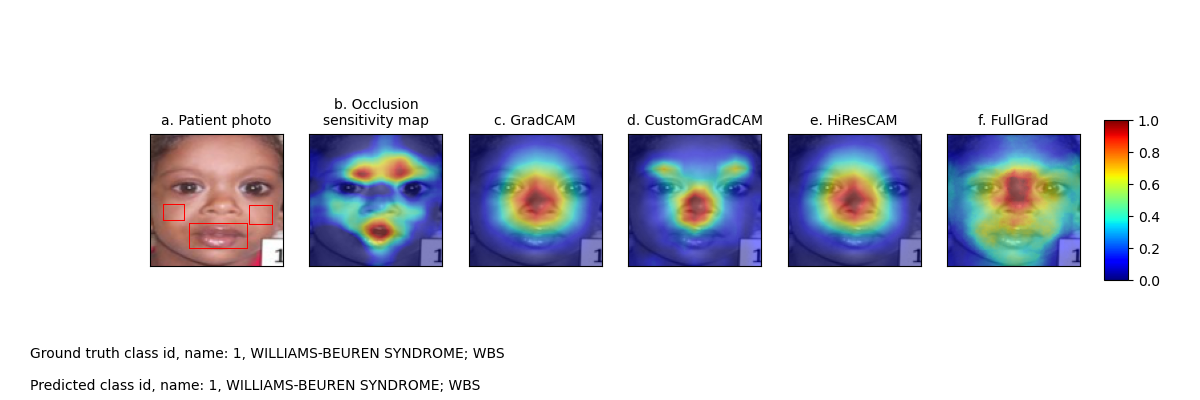
\includegraphics[width=\textwidth, trim = 1cm 2.50cm 1cm 2cm, clip]{chapter6/william/2_137.png}
		\caption{Patient with  WBS, and lips and cheeks specified as key features}
		\end{subfigure}
		\begin{subfigure}[t]{1\textwidth}
		\centering
		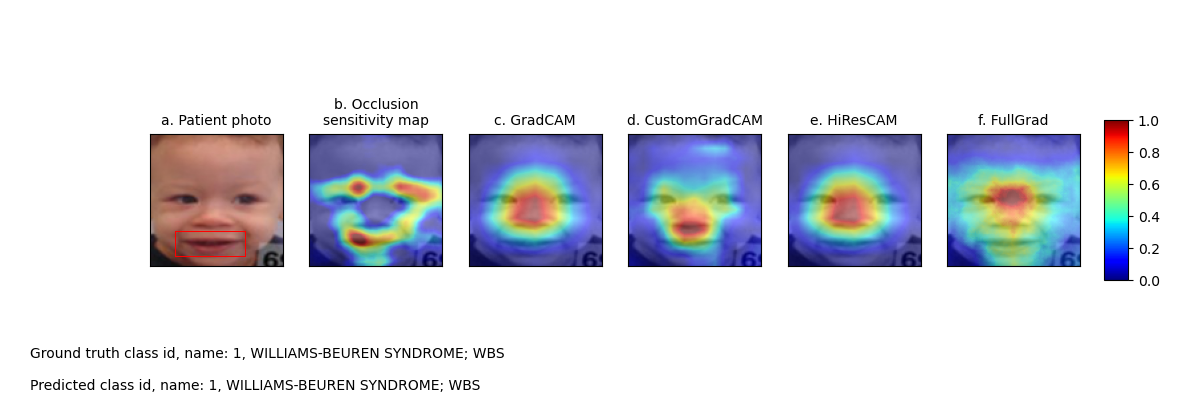
\includegraphics[width=\textwidth, trim = 1cm 2.50cm 1cm 2cm, clip]{chapter6/william/6_76.png}
		\caption{Patient with  WBS, and lips specified as the key feature}
		\end{subfigure}
		\caption[Attribution maps of instances in which clinician's attention regions differ from that of the classifier model]{Attribution maps of instances in which clinician's attention regions differ from that of the classifier model. Key features specified by the clinician are boxed in red. Method chosen for the first instance is boxed in green color.}
	\end{figure}
	
    
    
    \subsection{Other Observations}
    
    
    \subsection{Evaluation Summary}
    
    \section{Experiment B. Composite Face Generation}
    Figure \ref{} contains composite faces of the top-ten syndrome classes by sample strength in 
    
    
    
    
    
    
    
    
    \section{Experiment C. Syndrome-wise Attribution Map Generation}


	\section{Experiment D. Dataset Imbalance - Explanation Quality Analysis}

    \section{Evaluation Summary}


\end{document}
